% Original handout vector figure with native, editable TikZ annotations.
\documentclass[10pt,a4paper,landscape]{article}
\usepackage[margin=7mm]{geometry}
\usepackage[T1]{fontenc}
\renewcommand{\rmdefault}{ptm}
\usepackage{amsmath,amssymb,booktabs,graphicx,tikz}
\usetikzlibrary{arrows.meta}
\pagestyle{empty}
\setlength{\parindent}{0pt}
\setlength{\parskip}{3pt}
\definecolor{ink}{HTML}{243746}
\definecolor{acol}{HTML}{D17B14}
\definecolor{dcol}{HTML}{963D98}
\definecolor{xcol}{HTML}{1765B0}
\definecolor{ycol}{HTML}{C43C39}
\definecolor{zcol}{HTML}{22854E}
\newcommand{\xx}[1]{\textcolor{xcol}{#1}}
\newcommand{\yy}[1]{\textcolor{ycol}{#1}}
\newcommand{\zz}[1]{\textcolor{zcol}{#1}}
\newcommand{\orig}[3]{\fill[ink] (#1) circle (2.0bp);\draw[ink!70,line width=.45pt] (#1)--(#2);\node[fill=white,inner sep=1.4pt,text=ink,font=\small] at (#2) {#3};}
\newcommand{\frameorig}[7]{%
\fill[ink] (#1) circle (2.0bp);
\draw[ink!70,line width=.45pt] (#1)--(#2);
\node[fill=white,draw=ink!40,rounded corners=1pt,inner sep=2.4pt,text=ink,font=\footnotesize] at (#2)
{\begin{tabular}{@{}c@{}}#3\\\xx{$x_{#4}=#5$}\quad\yy{$y_{#4}=#6$}\\\zz{$z_{#4}=#7$}\end{tabular}};}
\newcommand{\via}[3]{\draw[dcol,fill=white,line width=.8pt] (#1) circle (2bp);\draw[dcol!70,line width=.45pt] (#1)--(#2);\node[fill=white,inner sep=1.4pt,text=dcol,font=\small] at (#2) {#3};}
\newcommand{\dimtag}[3]{\node[fill=white,inner sep=1.2pt,text=#1,font=\small] at (#2) {#3};}
\newcommand{\triad}[8]{%
\begin{tikzpicture}[x=18mm,y=18mm,baseline=(current bounding box.center),>=Stealth]
\path[use as bounding box] (-.65,-.64) rectangle (.76,.75);
\node[font=\scriptsize,text=ink] at (0,.65) {$i=#1$};
\draw[->,xcol,line width=.7pt] (0,0)--(#2,#3) node[font=\small,anchor=#8] {$x_i$};
\draw[->,ycol,line width=.7pt] (0,0)--(#4,#5);
\ifdim #5pt<0pt
\node[font=\small,ycol,below] at (#4,#5) {$y_i$};
\else
\node[font=\small,ycol,above] at (#4,#5) {$y_i$};
\fi
\draw[->,zcol,line width=.7pt] (0,0)--(#6,#7) node[font=\small,right] {$z_i$};
\fill[ink] (0,0) circle (.7pt);
\end{tikzpicture}}
\begin{document}
{\fontsize{16}{18}\selectfont\bfseries\color{ink} Left leg: D-H origins, construction distances and axes}\par
{\small Original assignment Fig. 2 retained underneath. Added labels use $O_i$, $P_i$, $a_{i-1}^{\rm DH}$ and $d_i^{\rm DH}$; all listed lengths are in mm.}\par\vspace{1mm}
\begin{minipage}[t]{0.485\textwidth}
\vspace{0pt}
\centering
\begin{tikzpicture}[x=1bp,y=-1bp,>=Stealth]
\path[use as bounding box] (-60,-5) rectangle (306,415);
\node[anchor=north west,inner sep=0,opacity=.9] at (0,0) {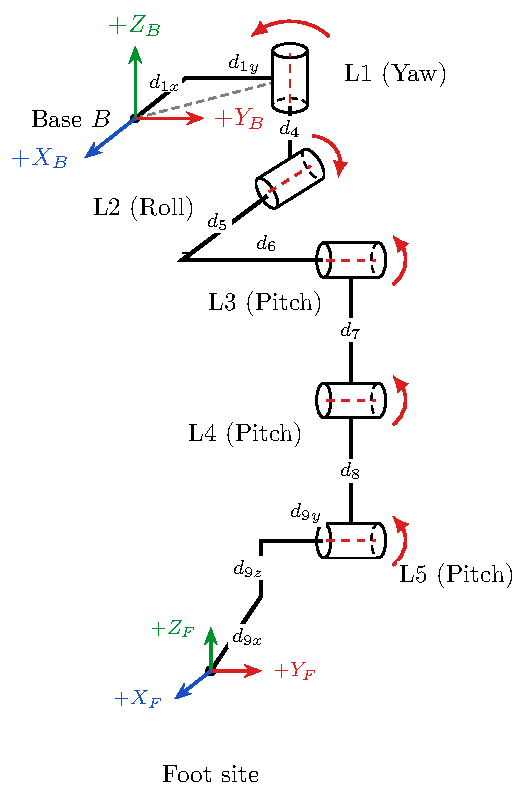
\includegraphics[width=255bp]{../assets/assignment_left_original.pdf}};
\coordinate (O0) at (65,56);
\coordinate (P1) at (139,38);
\coordinate (O1) at (139,83);
\coordinate (O2) at (76.75,124.5);
\coordinate (O3) at (168.5,124.5);
\coordinate (O4) at (168.5,191.5);
\coordinate (P5) at (168.5,259.5);
\coordinate (O5) at (125.5,259.5);
\coordinate (P6) at (101.5,277.5);
\coordinate (O6) at (101.5,322);
% Unsigned axis lines follow the source drawing's schematic joint axes.
% Positive directions are specified separately in B; the original drawing
% does not have one consistent, calibrated projection for every joint.
\draw[gray,densely dashed,line width=.6pt] (139,27)--(139,95);
\draw[gray,densely dashed,line width=.6pt] (68,130.33)--(158,70.33);
\draw[gray,densely dashed,line width=.6pt] (70,124.5)--(190,124.5);
\draw[gray,densely dashed,line width=.6pt] (151,191.5)--(192,191.5);
\draw[gray,densely dashed,line width=.6pt] (115,259.5)--(185,259.5);
% MDH construction routes. Offset dimension lines are joined to their
% true annotated endpoints by fine extension lines.
\draw[->,acol,line width=1.15pt] (O0)--(P1);
\dimtag{acol}{97,36}{$a_0^{\rm DH}$}
\draw[dcol!65,line width=.4pt] (P1)--(154,38) (O1)--(154,83);
\draw[->,dcol,line width=1.15pt] (154,38)--(154,83);
\dimtag{dcol}{184,61}{$d_1^{\rm DH}$}
\draw[->,dcol,line width=1.1pt] (O1)--(O2);
\dimtag{dcol}{104,93}{$d_2^{\rm DH}$}
\draw[->,dcol,line width=1.1pt] (O2)--(O3);
\dimtag{dcol}{123,132}{$d_3^{\rm DH}$}
\draw[acol!65,line width=.4pt] (O3)--(187,124.5) (O4)--(187,191.5);
\draw[->,acol,line width=1.15pt] (187,124.5)--(187,191.5);
\dimtag{acol}{213,165}{$a_3^{\rm DH}$}
\draw[acol!65,line width=.4pt] (O4)--(187,191.5) (P5)--(187,259.5);
\draw[->,acol,line width=1.15pt] (187,191.5)--(187,259.5);
\dimtag{acol}{213,226}{$a_4^{\rm DH}$}
\draw[dcol!65,line width=.4pt] (P5)--(168.5,271) (O5)--(125.5,271);
\draw[->,dcol,line width=1.1pt] (168.5,271)--(125.5,271);
\dimtag{dcol}{148,283}{$d_5^{\rm DH}$}
\draw[acol!65,line width=.4pt] (O5)--(112.5,256.5) (P6)--(88.5,274.5);
\draw[->,acol,line width=1.1pt] (112.5,256.5)--(88.5,274.5);
\dimtag{acol}{67,267}{$a_5^{\rm DH}$}
\draw[dcol!65,line width=.4pt] (P6)--(85,277.5) (O6)--(85,322);
\draw[->,dcol,line width=1.1pt] (85,277.5)--(85,322);
\dimtag{dcol}{54,299}{$d_6^{\rm DH}$}
% Origins and intermediate points. Leaders are deliberately distinct
% from the original cylinder centres.
\orig{O0}{17,28}{\shortstack{$O_0=O_B$\\\scriptsize Frame 0: see axis key}}
\via{P1}{200,8}{$P_1$}
\frameorig{O1}{249,85}{$O_1=P_2$}{1}{+Y}{-X}{+Z}
\frameorig{O2}{-10,132}{$O_2=P_3$}{2}{+Z}{-Y}{+X}
\frameorig{O3}{249,140}{$O_3$}{3}{-Z}{-X}{+Y}
\frameorig{O4}{249,192}{$O_4=P_4$}{4}{-Z}{-X}{+Y}
\via{P5}{243,249}{$P_5$}
\frameorig{O5}{19,245}{$O_5$}{5}{+X}{-Z}{+Y}
\via{P6}{28,283}{$P_6$}
\frameorig{O6}{240,335}{$O_6=S$}{6}{+X}{+Y}{+Z}
\node[align=left,text=ink,font=\footnotesize,anchor=north west] at (-30,388)
{Filled dots: selected D-H origins. Open dots: intermediate $P_i$.\\
Boxed XYZ keys give directions in base $B$, not page directions.\\
Arrow paths show construction order on the original schematic.};
\end{tikzpicture}
\end{minipage}\hfill
\begin{minipage}[t]{0.50\textwidth}
\vspace{0pt}
\color{ink}\small
\textbf{Read each row as two translations}
\[
O_{i-1}\ \xrightarrow[\text{along }+x_{i-1}]{\color{acol}a_{i-1}^{\rm DH}}\ P_i
\ \xrightarrow[\text{along }+z_i]{\color{dcol}d_i^{\rm DH}}\ O_i.
\]
Negative values mean travel opposite to the stated positive axis.
\par\vspace{1mm}
\centering
\renewcommand{\arraystretch}{1.10}
\begin{tabular}{ccll}
\toprule
Row & Route & \textcolor{acol}{$a_{i-1}^{\rm DH}$} & \textcolor{dcol}{$d_i^{\rm DH}$}\\
\midrule
1 & $O_0\to P_1\to O_1$ & $+39.8246$ along $x_0$ & $-0.0741$ along $+Z$\\
2 & $O_1=P_2\to O_2$ & $0$ & $-16.060$ along $+X$\\
3 & $O_2=P_3\to O_3$ & $0$ & $+74.150$ along $+Y$\\
4 & $O_3\to P_4=O_4$ & $+78.650$ along $-Z$ & $0$\\
5 & $O_4\to P_5\to O_5$ & $+78.650$ along $-Z$ & $-19.750$ along $+Y$\\
6 & $O_5\to P_6\to O_6$ & $+0.500$ along $+X$ & $-36.225$ along $+Z$\\
\bottomrule
\end{tabular}
\par\vspace{2mm}\raggedright
\textbf{Positive coordinate axes at every origin (zero pose)}
\par\centering
\begin{tabular}{clll}
\toprule
Frame & \xx{$+x_i$} & \yy{$+y_i$} & \zz{$+z_i$}\\
\midrule
0 & \xx{$-sX+cY$} & \yy{$-cX-sY$} & \zz{$+Z$}\\
1 & \xx{$+Y$} & \yy{$-X$} & \zz{$+Z$}\\
2 & \xx{$+Z$} & \yy{$-Y$} & \zz{$+X$}\\
3, 4 & \xx{$-Z$} & \yy{$-X$} & \zz{$+Y$}\\
5 & \xx{$+X$} & \yy{$-Z$} & \zz{$+Y$}\\
6 (site) & \xx{$+X$} & \yy{$+Y$} & \zz{$+Z$}\\
\bottomrule
\end{tabular}
\par\raggedright
$X,Y,Z$ denote the base axes; $s=19/\sqrt{19^2+35^2}$,
$c=35/\sqrt{19^2+35^2}$. All frames satisfy $x_i\times y_i=z_i$.
\par\centering
\begin{tabular}{ccc}
\triad{0}{.4}{.08}{.06}{.38}{0}{.25}{west}&
\triad{1}{.4}{0}{.30}{.23}{0}{.36}{west}&
\triad{2}{0}{.36}{-.4}{0}{-.30}{-.23}{south}\\[-2mm]
\triad{3,4}{0}{-.36}{.30}{.23}{.4}{0}{north}&
\triad{5}{-.30}{-.23}{0}{-.36}{.4}{0}{east}&
\triad{6}{-.30}{-.23}{.4}{0}{0}{.36}{east}
\end{tabular}
\par\raggedright\footnotesize
\textbf{Origin placement.} $O_1$ is the yaw/roll axis intersection;
$O_2$ is the roll/hip-pitch intersection. They are not the drawn cylinder
centres. $P_1$ is a schematic yaw-axis reference at base height.
For row 6, the construction takes the small $a_5$ step first, then $d_6$.
\par
\textbf{Source drawing versus signed geometry.} The original is not to scale
and its joint symbols do not share a calibrated 3-D projection. Gray joint-axis
lines on the drawing are \emph{unoriented}; the table and triads define the exact
positive directions. Original labels $d_4,d_5,\ldots$ are handout dimension names,
not D-H row numbers. In particular, $d_1^{\rm DH}=-0.0741$ is the selected
origin's net height, not the CAD yaw-to-roll anchor separation.
\end{minipage}
\end{document}
